\section{Steering Model of the Vehicle}\label{sec:SteeringModel}
\todo{rewrite}The following section will describe and model the steering of the vehicle. The relationship between the vehicle's speed, the angle of the servo, the brakes, and the actual steering of the vehicle will be examined. A overview of the braking system can be seen in \figref{steeringMechanical}.

 \begin{figure}[H]
 	\centering
 	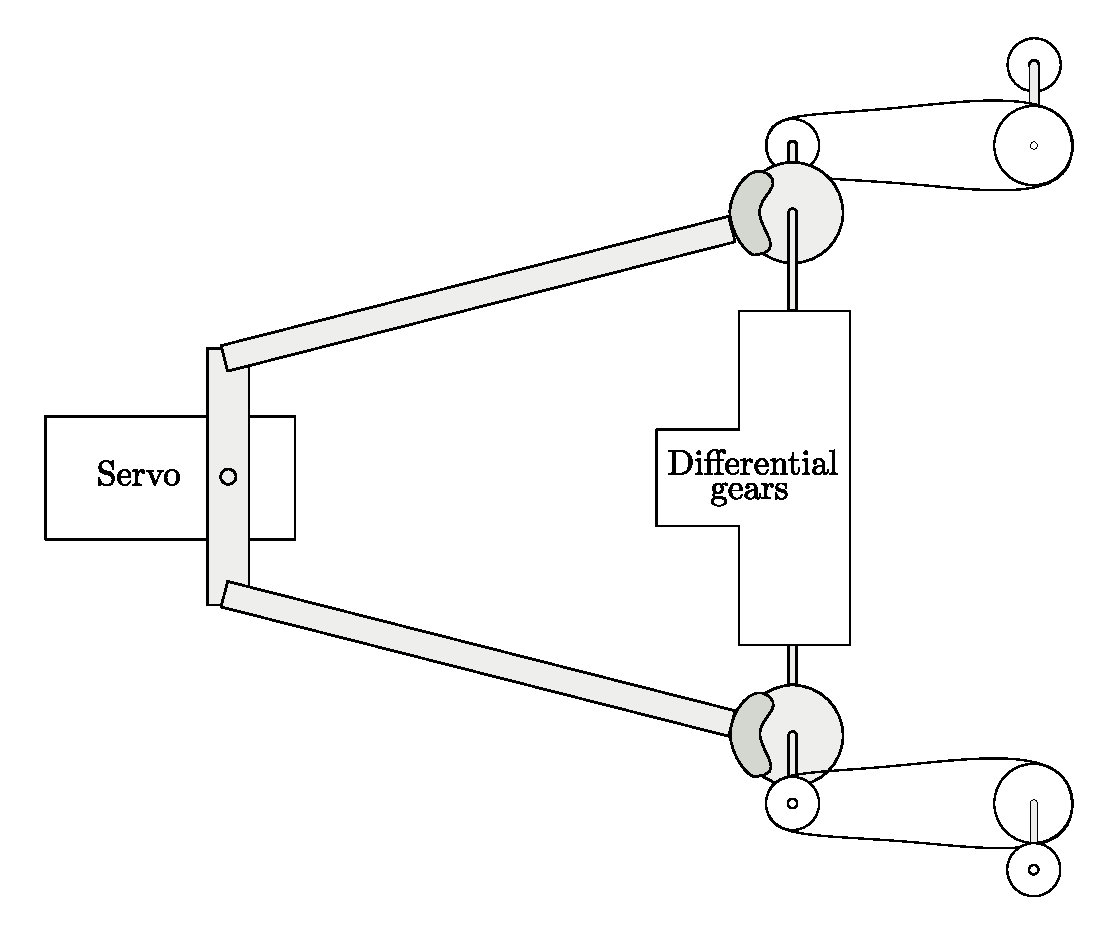
\includegraphics[scale=0.6]{figures/steeringMechanical.pdf}
 	\caption{Mechanical drawing of the steering}
 	\label{steeringMechanical}
 \end{figure}

When the servo turns one way, it push the brake pads on the brake disc, to add a friction. The differential gears will transfer the power from one belt to the other if one brake is triggered.

\subsection{Directional model}
As the steering system contains many moving parts, it would be advantageous to start with a simple model, verifying it, and iterate until it is satisfactory. 

The first model considered can be seen on \figref{basicSteering}.

\begin{figure}[H]
	\centering
	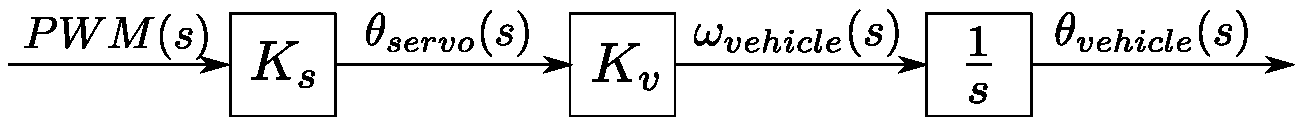
\includegraphics[width=0.8\textwidth]{figures/basicSteeringModel.pdf}
	\caption{A basic steering model}
	\label{basicSteering}
\end{figure}
 
As described in \secref{Servo}, the angle of the servo is proportional to a pulse width modulated signal on it's control input. The pulse width is therefore chosen as the input in this model. This is multiplied by a constant, $\text{K}_\text{s}$, which translates the pulse width to an angle of the servo.
If the velocity of the vehicle is assumed constant, the rate of change of the direction must be a function of the servo angle, and a constant, $\text{K}_\text{c}$, representing the speed of the vehicle.
The rate of change is integrated over time, resulting in a direction. 

\subsection{Expansion of the Directional Model}

The model can be extended to include the time delay in the servo. According to \todo{ref}, the servo is controlled by a PWM signal, with a period of 30 ms. This means, that it will not be possible to update the servo angle continuously, but only in discrete time steps of 30 ms. These steps will be implemented in the model as a delay.



According to \todo{ref slide} a small time delay can be modelled as:
$\frac{1}{\lambda\cdot\text{s}+1}$ \todo{add more equations from the slide}

\begin{figure}[H]
	\centering
	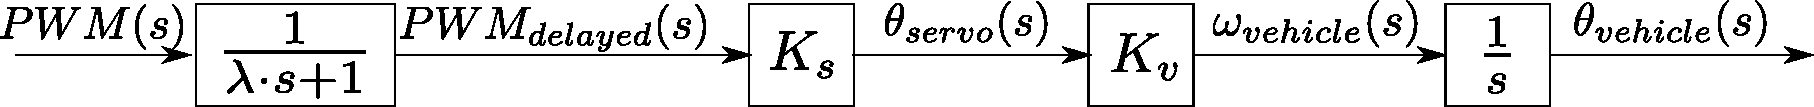
\includegraphics[width=0.8\textwidth]{figures/basicSteeringModelWithDelay.pdf}
	\caption{A basic steering model}
	\label{basicSteeringWithDelay}
\end{figure}

\subsection{Line Following Model}
As the vehicle has to follow a predetermined routwe, a direction alone is not enough. As seen on \figref{SteeringDeviation}, any change of direction caused by a disturbance, will cause a deviation from the planned line from A to B.

\begin{figure}[H]
	\centering
	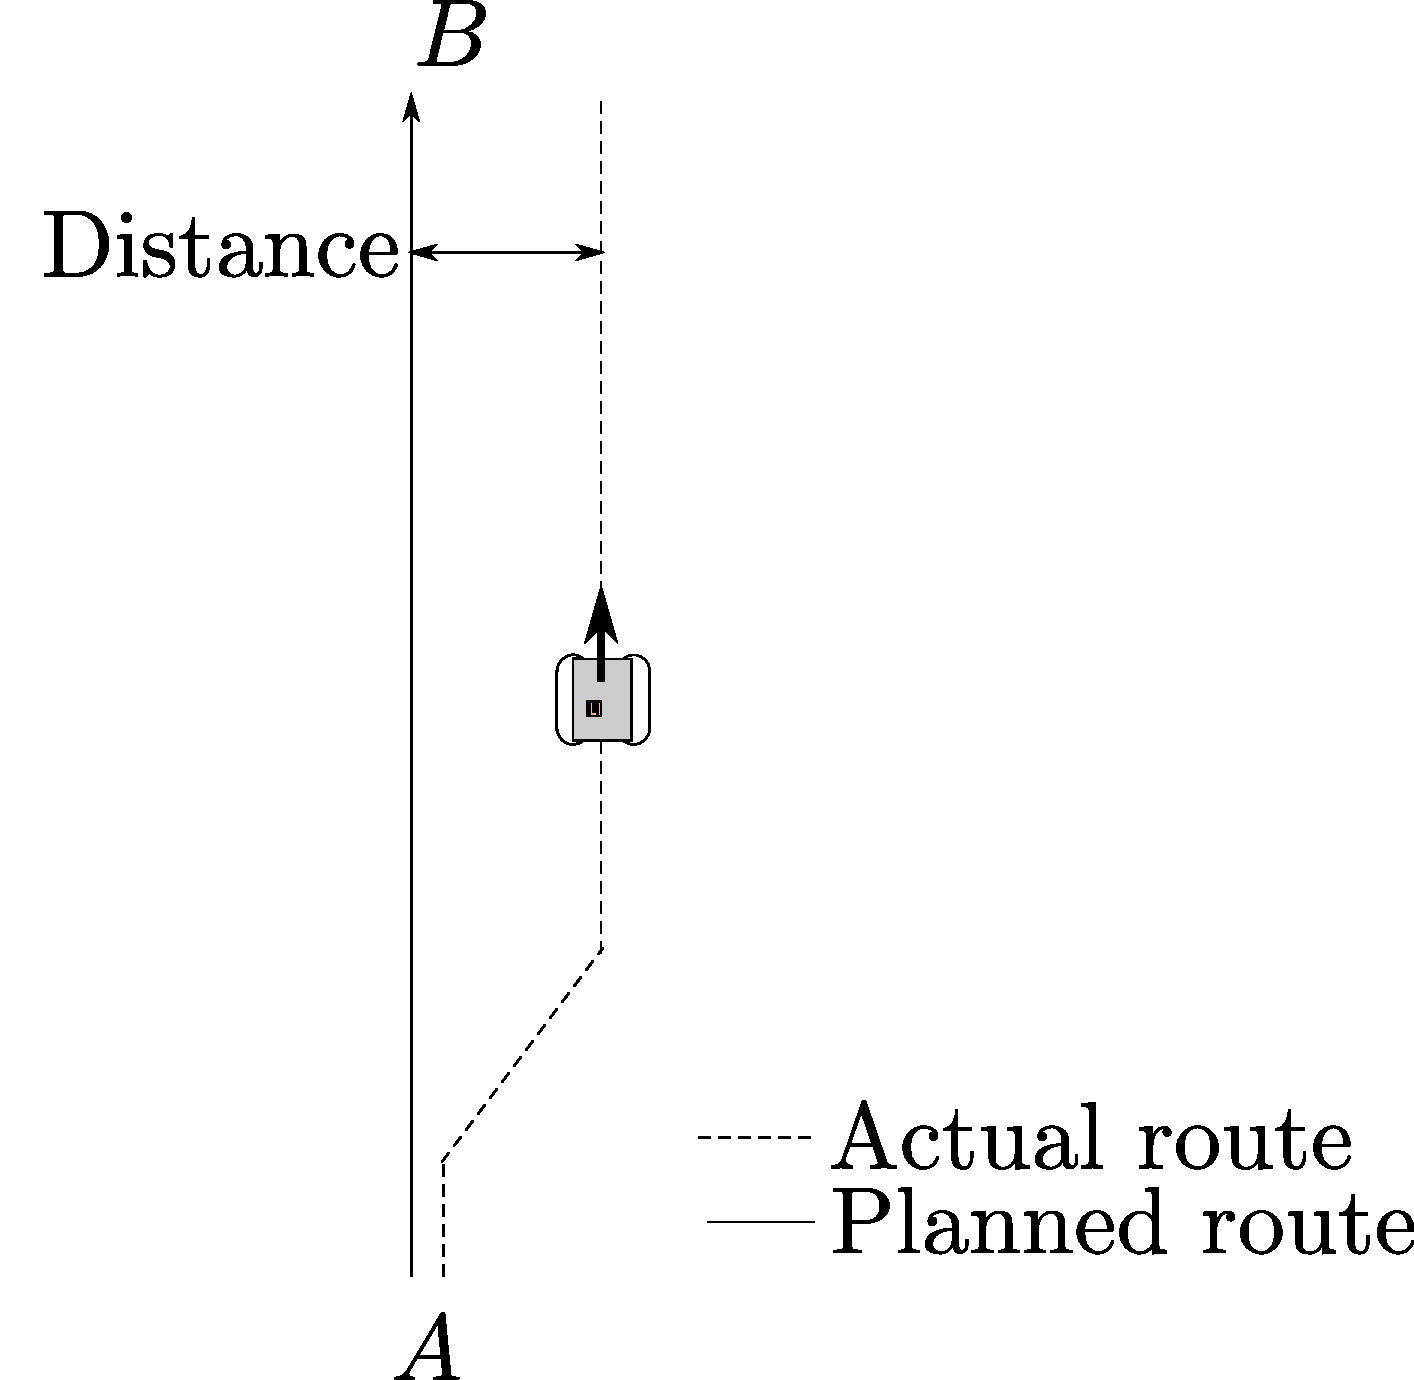
\includegraphics[width=0.8\textwidth]{figures/steeringDeviation.pdf}
	\caption{Consequence of using directional control alone}
	\label{SteeringDeviation}
\end{figure}

How large the deviation will be must depend on the erroneous angle, the speed, and the time it takes to correct the error. Assuming the speed is constant, the error can be described as an integration of the error angle over time.






%Servoen tilføjer en ekstra pol til systemet og da vi ved at servoen giver et samplingsdelay. kan stille dens system op som det som står slidet.

%Det er fordel at kunne holde polen i servoen langt væk fra polen i directional modelen, for så kan vi se bort den pol som er servoen. (ligesom vi har gjort i velocity model, vi har lavet et andet ordens system om til et første ordens.)

%tau i servoen er 0.03 da servoens samples med 30 ms, se servoafsnit.

%Man burde kunne lave en model uden en controller, men da systemet er meget ulignært er der valgt at implementere en controller order to stabilise the measurements. 

%\subsection{Order Of The System}
%As seen on \figref{plotStepResponseSteering}, the step response for the steering test has a direct rise of the angle after the step, typical of a first order system.

%Second or first order, if it is second the black box should be expanded, if it is first there is no need because then we have all the parameters from the test.
 
 
%  appendix
 
% show that it's a first order system\\
% then integrator\\
% then is linear(multiples values) the speed of turning at different PWM angle of the servo?
